\documentclass[paper,twocolomn]{geophysics}
%\documentclass[manuscript]{geophysics}
%\documentclass[manuscript,endfloat]{geophysics}
\usepackage{amsmath,amssymb,amsfonts,graphicx,subfigure,bm,yfonts,hyperref,cleveref,xcolor}
\usepackage{rotating}
%\usepackage[outdir=./]{epstopdf}

\usepackage{multirow}


%%%%%%%%%                              DEFINITIONS START

\def\cpar{$C_{ij},\rho$ parameterization~}
\def\hpar{h-parameterization~}

\newcommand{\todo}[1]{{\textbf {\color{red} #1}}}
\newcommand{\done}[1]{{\bf {\color{green} #1}}}
\newcommand{\connect}{{\textbf{\color{red} $<-$ Connect $->$ }}}


\def\rmrk#1{{\textbf{[[#1]]}}}
\def\rmrkok#1{}
%\def\eqref#1{\ref{#1}}
\def\eqrf#1{equation~\eqref{eq:#1}}
%\def\eqref#1{equation~\ref{eq:#1}}
\def\eq{equation~}
\def\figref#1{Figure~\ref{fig:#1}}
\def\figrefp#1{(Figure~\ref{fig:#1})}

\def\fref#1{\ref{#1}}

\def\rhoK{\hat{\rho}}
\def\cK{\hat{c}}


%\def\rmrk#1{{[\textcolor[rgb]{0,0,0.8}{#1}]}} % [blue]
%\def\rmrkm#1{{\textbf{[[\textcolor[rgb]{{1.00,0.00,0.00}}{#1}]]}}}
% _____________________________________________________________________________
\def\mainauthor{Vladimir Kazei}
\def\coauthorb{Ekkehart Tessmer}
\def\coauthorc{}%Zedong Wu
\def\coauthora{Tariq Alkhalifah}
% - my definitions==============================================================================================

\def\DP{Diffraction-based radiation 
patterns }
\def\dP{diffraction-based radiation 
patterns }

\def\nt{N}
\newcommand{\Mod}[1]{\ (\mathrm{mod}\ #1)}
\def\dv{\mathbf{d}}
\def\Amat{\mathbb{A}}
\def\Rmat{\mathbb{R}}
\def\Umat{\mathbb{U}}
\def\Smat{\mathbb{S}}
\def\Vmat{\mathbb{V}}
\def\SF{R}
\def\xv{\mathbf{x}}
\def\mv{\mathbf{m}}
%\def\tmul{\otimes}
\def\tmul{}
\def\cv{\mathbf{c}}

\def\sp{\varsigma}
\def\spv{\bm{\sp}}
\def\gp{\xi}
\def\gpv{\bm{\gp}}

\newcommand{\nmz}[1]{\mathbf{\bar{\text{$#1$}}}}
%\def\nmz#1{\mathbf{\bar #1}}

\def\Uv{\mathbf{U}}
\def\kv{\mathbf{k}}
\def\sv{\mathbf{s}}
\def\svn{\mathbf{\bar{\sv}}}
\def\Sv{\mathbf{S}}
\def\Gv{\mathbf{G}}
\def\Cv{\mathbf{C}}
\def\ev{\mathbf{e}}
\def\gv{\mathbf{g}}
\def\gvn{\mathbf{\bar{\gv}}}
\def\Av{\mathbf{A}}
\def\Bv{\mathbf{B}}
\def\uv{\mathbf{u}}
\def\rv{\mathbf{r}}
\def\dxv{\Delta \mathbf{x}}
\def\Kv{\mathbf{K}}
\def \cost{ \cos \frac{\theta}{2}}
%\newcommand{\sdot}{\mathbf{\bullet}}

\newcommand{\sdot}{{WI-WS, \delta \mv}}

\newcommand{\inty}{\int\limits_{-\infty}^{+\infty}}
\newcommand{\intyt}{\inty\inty\inty}
\newcommand{\intyV}{\int\limits_{V}}

\def\Rp{\mathcal{R}}
\def\Dp{\mathcal{D}}
\def\Tp{\mathcal{T}}
%\def\Cp{\mathcal{C}}
\def\Sp{\mathcal{S}}

% - Tariq's definitions begin here ==============================================================================
\def\beq{\begin{eqnarray}}
\def\eeq{\end{eqnarray}}

\def\mmbx#1{{\mathbf{#1}}}

\def\phi{\varphi}

\def\Vv{\mmbx{V}}
\def\gammav{\pmb{\gamma}}
\def\epsv{\pmb{\eps}}
\def\deltav{\pmb{\delta}}
\def\etav{\pmb{\eta}}

\def\v{V}
\def\rhov{\pmb{\rho}}
\def\r{\mmbx{r}}
\def\k{\mmbx{k}}

\def\d{\text{d}}
\def\c{\mmbx{c}}
\def\e{\mmbx{e}}
\def\m{\mmbx{m}}
\def\x{\mmbx{x}}
\def\xs{\x_s}
\def\xr{\x_r}
\def\L{\mmbx{L}}
\def\p{\mmbx{p}}
\def\q{\mmbx{q}}

\def\La{{\cal L}}
\def\tf{\tilde{f}}
\def\tA{\tilde{A}}
\def\ttau{\tilde{\tau}}
\def\y{\mmbx{y}}
\def\z{\mmbx{z}}

\def\tm{\tilde{m}}
\def\tr{\tilde{r}}
\def\tw{\tilde{w}}
\def\tv{\tilde{v}}
\def\tp{\tilde{p}}
\def\tq{\tilde{q}}

\def\a{\mmbx{a}}
\def\H{\mmbx{H}}
\def\g{\mmbx{g}}
\def\W{\mmbx{W}}

\def\eps{\varepsilon}

\def\La{{\cal L}}

\def\tlambda{\tilde{\lambda}}
\def\tw{\tilde{w}}

\def\rvn{r_{v_n}}
\def\rvh{r_{v_h}}
\def\rrho{r_\rho}
\def\rdel{r_\delta}
\def\reta{r_\eta}
\def\reps{r_\eps}


\def\Re{{{\cal{R}}_e}}

\newcommand{\pd}[2]{\frac{\partial #1}{\partial #2}}

%==============================================end of Tariq's notation=========================================


%%%%%%%%%								DEFINITIONS END
\newcommand{\mylabel}[1]{\label{#1}}
\newcommand{\myrf}[1]{\ref{#1}}

%%\newcommand{\plot}[3]{
%	\begin{figure}
%		\center
%		\includegraphics[#2]{Fig/#1}
%		\caption{#3}
%		\label{fig:#1}
%	\end{figure}
%}

\newcommand{\aplot}[3]{
	\begin{figure}[htbp!]
		\center
		\includegraphics[#2]{#1}
		\caption{#3}
		\label{fig:#1}
	\end{figure}
}

\newcommand{\twplot}[3]{
	\begin{figure}
		\centering
		\subfigure[]{\includegraphics[width=0.4\columnwidth]{Fig/#1}
			\label{fig:#1}}
		\hspace*{-0.01\columnwidth}
		\subfigure[]{\includegraphics[width=0.55\columnwidth]{Fig/#2}
			\label{fig:#2}}
		\caption{#3}
		%\label{fig:#1}
	\end{figure}
}

\newcommand{\tplot}[4]{
	\begin{figure}
		\centering
		\subfigure[]{\includegraphics[width=0.3\columnwidth]{Fig/#1}
			\label{fig:#1}}
		\vspace*{-0.01\columnwidth}
		\subfigure[]{\includegraphics[width=0.3\columnwidth]{Fig/#2}
			\label{fig:#2}}
		\vspace*{-0.01\columnwidth}
		\subfigure[]{\includegraphics[width=0.3\columnwidth]{Fig/#3}
			\label{fig:#3}}
		\caption{#4}
		\label{fig:#1_#3}\label{fig:#1_Full}
	\end{figure}
}
\newcommand{\tplott}[4]{
	\begin{figure}
		\centering
		\subfigure[]{\includegraphics[width=0.2\columnwidth]{Fig/#1}
			\label{fig:#1}}
		\vspace*{-0.01\columnwidth}
		\subfigure[]{\includegraphics[width=0.4\columnwidth]{Fig/#2}
			\label{fig:#2}}
		\vspace*{-0.01\columnwidth}
		\subfigure[]{\includegraphics[width=0.3\columnwidth]{Fig/#3}
			\label{fig:#3}}
		\caption{#4}
		\label{fig:#1_#3}\label{fig:#1_Full}
	\end{figure}
}
\newcommand{\tplotv}[4]{
	\begin{figure}
		\centering
		\subfigure[]{\includegraphics[width=0.49\columnwidth]{Fig/#1}
			\label{fig:#1}}
		\vspace*{-0.01\columnwidth}
		\subfigure[]{\includegraphics[width=0.49\columnwidth]{Fig/#2}
			\label{fig:#2}}
		\vspace*{-0.01\columnwidth}
		\subfigure[]{\includegraphics[width=0.49\columnwidth]{Fig/#3}
			\label{fig:#3}}
		\caption{#4}
		\label{fig:#1_#3}\label{fig:#1_Full}
	\end{figure}
}

\newcommand{\ffplot}[5]{
	\begin{figure}
		\centering
		\subfigure[]{\includegraphics[height=0.47\columnwidth]{Fig/#1}
			\label{fig:#1}}
		\hspace*{0.01\columnwidth}
		\subfigure[]{\includegraphics[height=0.47\columnwidth]{Fig/#2}
			\label{fig:#2}}
		\hspace*{-0.01\columnwidth}
		\subfigure[]{\includegraphics[height=0.47\columnwidth]{Fig/#3}
			\label{fig:#3}}
		\hspace*{0.01\columnwidth}
		\subfigure[]{\includegraphics[height=0.47\columnwidth]{Fig/#4}
			\label{fig:#4}}
		\caption{#5}
		\label{fig:#1:#4}\label{fig:#1_Full}
		\vspace*{-0.03\columnwidth}
	\end{figure}
}

\newcommand{\fplot}[5]{
	\begin{figure}
		\centering
		\subfigure[]{\includegraphics[height=0.27\columnwidth]{Fig/#1}
			\label{fig:#1}}
		\hspace*{0.01\columnwidth}
		\subfigure[]{\includegraphics[height=0.27\columnwidth]{Fig/#2}
			\label{fig:#2}}
		\hspace*{-0.01\columnwidth}
		\subfigure[]{\includegraphics[height=0.27\columnwidth]{Fig/#3}
			\label{fig:#3}}
		\hspace*{0.01\columnwidth}
		\subfigure[]{\includegraphics[height=0.27\columnwidth]{Fig/#4}
			\label{fig:#4}}
		\caption{#5}
		\label{fig:#1:#4}\label{fig:#1_Full}
		\vspace*{-0.03\columnwidth}
	\end{figure}
}

\newcommand{\splot}[7]{
	\begin{figure}
		\centering
		\subfigure[]{\includegraphics[height=0.27\columnwidth]{Fig/#1}
			\label{fig:#1}}
		\hspace*{0.01\columnwidth}
		\subfigure[]{\includegraphics[height=0.27\columnwidth]{Fig/#2}
			\label{fig:#2}}
		\hspace*{-0.01\columnwidth}
		\subfigure[]{\includegraphics[height=0.27\columnwidth]{Fig/#3}
			\label{fig:#3}}
		\hspace*{0.01\columnwidth}
		\subfigure[]{\includegraphics[height=0.27\columnwidth]{Fig/#4}
			\label{fig:#4}}
		\subfigure[]{\includegraphics[height=0.27\columnwidth]{Fig/#5}
			\label{fig:#5}}
		\subfigure[]{\includegraphics[height=0.27\columnwidth]{Fig/#6}
			\label{fig:#6}}
		\caption{#7}
		\label{fig:#1:#6}\label{fig:#1_Full}
		\vspace*{-0.03\columnwidth}
	\end{figure}
}

\newcommand{\fiPlot}[6]{
	\begin{figure}
		\centering
		\subfigure[]{\includegraphics[width=0.31\columnwidth]{Fig/#1}
			\label{fig:#1}}
		\hspace*{-0.01\columnwidth}
		\subfigure[]{\includegraphics[width=0.31\columnwidth]{Fig/#2}
			\label{fig:#2}}
		\hspace*{-0.01\columnwidth}
		\subfigure[]{\includegraphics[width=0.31\columnwidth]{Fig/#3}
			\label{fig:#3}}
		\hspace*{-0.01\columnwidth}
		\subfigure[]{\includegraphics[width=0.33\columnwidth]{Fig/#4}
			\label{fig:#4}}
		\subfigure[]{\includegraphics[width=0.33\columnwidth]{Fig/#5}
			\label{fig:#5}}
		\caption{#6}
		\label{fig:#1:#5}\label{fig:#1_Full}
	\end{figure}
}

\newcommand{\dplot}[3]{
	\begin{figure}
		\centering
		\subfigure[]{\includegraphics[height=0.45\columnwidth]{Fig/#1}
			\label{fig:#1}}
		\hspace*{-0.01\columnwidth}
		\subfigure[]{\includegraphics[height=0.45\columnwidth]{Fig/#2}
			\label{fig:#2}}
		\vspace*{-0.01\columnwidth}
		\caption{#3}
		\label{fig:#1:#2}\label{fig:#1_Full}
	\end{figure}
}

\newcommand{\ddplot}[3]{
	\begin{figure}
		\centering
		\subfigure[]{\includegraphics[width=0.7\columnwidth]{Fig/#1}
			\label{fig:#1}}
		\hspace*{-0.01\columnwidth}
		\subfigure[]{\includegraphics[width=0.99\columnwidth]{Fig/#2}
			\label{fig:#2}}
		\vspace*{-0.01\columnwidth}
		\caption{#3}
		\label{fig:#1_#2}\label{fig:#1_Full}
	\end{figure}
}

\def\ewidth{0.4}


\newcommand{\eplot}[9]{
	\begin{figure}
		\centering
		\subfigure[]{\includegraphics[width=\ewidth\columnwidth]{Fig/#1}
			\label{fig:#1}}
		\hspace*{-0.01\columnwidth}
		\subfigure[]{\includegraphics[width=\ewidth\columnwidth]{Fig/#2}
			\label{fig:#2}}
		\hspace*{-0.01\columnwidth}
		\subfigure[]{\includegraphics[width=\ewidth\columnwidth]{Fig/#3}
			\label{fig:#3}}
		\hspace*{-0.01\columnwidth}
		\subfigure[]{\includegraphics[width=\ewidth\columnwidth]{Fig/#4}
			\label{fig:#4}}
		\hspace*{-0.01\columnwidth}
		\subfigure[]{\includegraphics[width=\ewidth\columnwidth]{Fig/#5}
			\label{fig:#5}}
		\hspace*{-0.01\columnwidth}
		\subfigure[]{\includegraphics[width=\ewidth\columnwidth]{Fig/#6}
			\label{fig:#6}}
		\hspace*{-0.01\columnwidth}
		\subfigure[]{\includegraphics[width=\ewidth\columnwidth]{Fig/#7}
			\label{fig:#7}}
		\hspace*{-0.01\columnwidth}
		\subfigure[]{\includegraphics[width=\ewidth\columnwidth]{Fig/#8}
			\label{fig:#8}}
		\caption{#9}
		%\label{fig:#1}
	\end{figure}
}


\graphicspath{{./Fig/}}

\begin{document}

\title{Seismic waveform inversion by deep learning: \\
	 velocity logs from multi-CMP gathers}

\renewcommand{\thefootnote}{\fnsymbol{footnote}} 

\author{Vladimir Kazei\footnotemark[1], Oleg Ovcharenko, Pavel Plotnitskii, Daniel Peter, Xiangliang Zhang \& Tariq Alkhalifah}
\address{
\footnotemark[1] KAUST, Saudi Arabia}
\date{\today}

\footer{submitted to Geophysics}
\lefthead{Kazei et al.}
\righthead{\emph{Seismic logs by CNN}}

\maketitle

\begin{abstract}
Building realistic and reliable models of the subsurface is the primary goal of seismic imaging.
%
Full-waveform inversion (FWI) allows to accommodate arbitrary physics and complexity that modeling can handle into seismic imaging to deliver the highest resolution possible.
  %
FWI is a local optimization technique and needs good initial model to start with.
  %
In order to estimate uncertainty in FWI several initial models are necessary.
%
We construct an ensamble of convolutional neural networks (CNN) to build velocity models directly from the data. 
 %
 %
CNNs are trained to map the seismic data directly into velocity logs. This allows to integrate the well data and to simplify the mapping by using the regularity of active seismic acquisition. 
%
The main feature of our approach is the usage of multiple CMP neigboring data in order to predict log at a given location. This allows us to accommodate larger dips that can be present in the subsurface then when using single CMP gathers. At the same time we still benefit from the regularity of sampling in seismic exploration.  
\end{abstract}

%% figure naming convention:
%(train/test)_(prefix(singleCMP/multiCMP))_{folder(for train: ""=x1,x2,x3:marmvel1D, marmvel1D_distorted,marmvel,overthrust1D,overthrust2D)}_{inverted/true/X_scaled}

\section{Introduction}
% what is the problem? FWI needs better starting model
% why FWI?
Seismic imaging and inversion is suffering from fundamental ambiguities such as lack of ultra-low frequencies in the data and ultra-long offsets. Thus ultimately results in the well-known gap in the intermediate wavenumber illumination of the subsurface models \citep{claerbout1985, mora1989, sirgue2004, alkhalifahFullmodelWavenumberInversion2016, kazei2016, kazei2018, yao2019extraction}. In most cases this gap is significant and causes difficulties while building smooth background models.

% solutions?
%\todo{Rephrase the paragraph} %FWI turned out to be so powerful and the problem of the lack of low frequencies in common exploration surveys is so challenging that possible solutions have been under development for decades.

From the algorithmic point of view the most straight forward solution would be to acquire new data. It is the most robust, already lead to major impact on exploration \citep[e.g.][]{fons2013} yet it is the most expensive, so the numerous methods have been developed to tackle the issue on the seismic data processing/inversion side. %We will split them into three generations.
% misfits
Conventional treatment of the lack of low wavenumber information is through changing the misfit functionals in full-waveform inversion \citep[e.g.][]{luo1991wave, bozdag2011, choi2012, leeuwen2013}. 
% gradients
Gradient filtering and conditioning \citep{ravaut2004multiscale, alkhalifah2015full, kazei2016, ovcharenko2018, ruan2018global} and closely related regularization techniques \citep{esserTotalvariationRegularizationStrategies2016, kazeiSaltbodyInversionMinimum2017, operto2018role, kalita2019regularized} is another way to approach the problem. All the methods listed above are rather intensive computationally.

% deep learning
Alternatively low wavenumber information can to some extent be inferred directly from the data in form of artificial low frequencies \citep{ovcharenkoNeuralNetworkBased2017,ovcharenkoLowFrequencyDataExtrapolation2018, ovcharenko2019deep, jin2018learn, kazei2019realistically} or low-dimensional models \citep[e.g.][]{polo2018}. The beauty of deep learning application in seismic inversion and velocity model building is that while training can be very computationally intensive, the application of the trained neural network is computationally very cheap \figref{learningParadigm} shows a speculative comparison of different seismic model building tools.
The ability to apply the network fast can also help to analyze uncertainty in full-waveform inversion coming from the initial model.
  
\begin{figure}
	\centering
	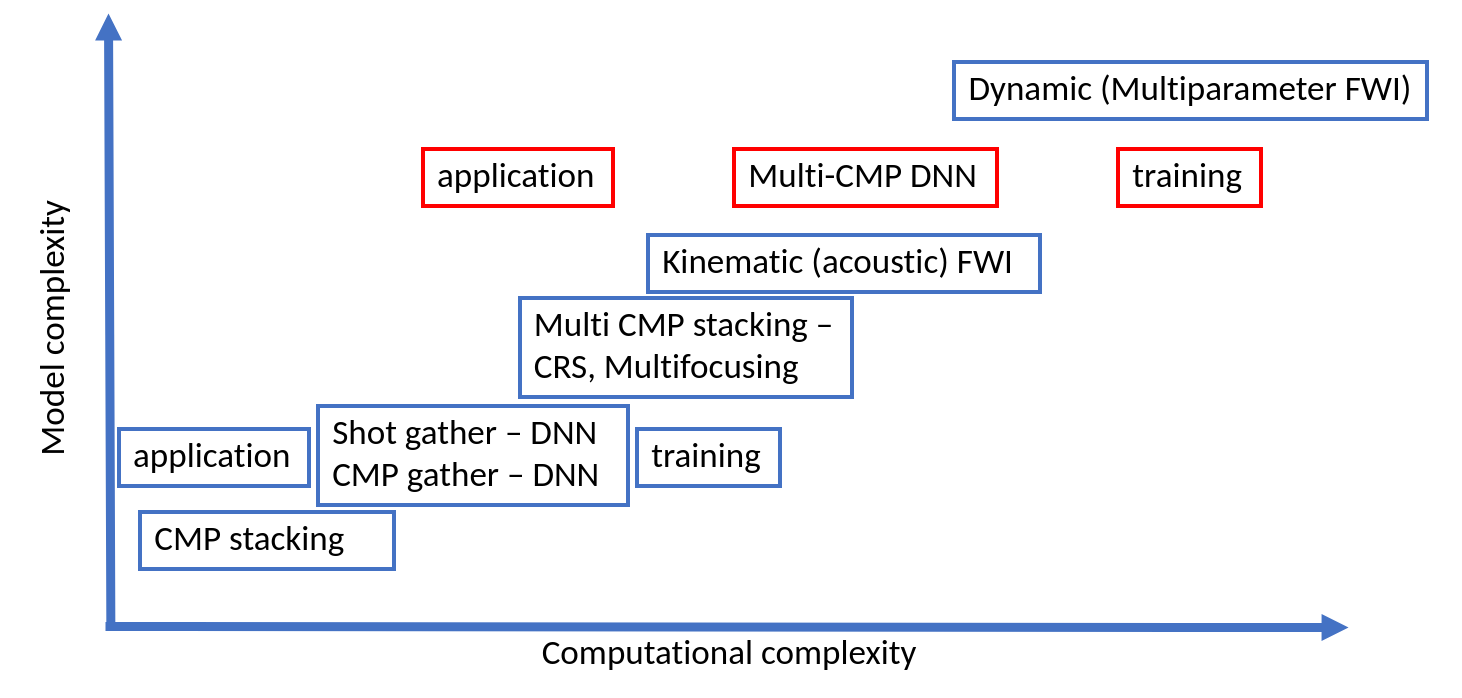
\includegraphics[width=0.9\linewidth]{Fig/learningParadigm}
	\caption{Deep learning is rather intensive in the training part, however the application of the trained deep neural network (DNN) is nearly instant}
	\label{fig:learningParadigm}
\end{figure}

% what shall we change?
Full waveform based methods listed above usually do not exploit the regularity of active seismic exploration sampling. Deep learning on the other hand can infer mapping for seismic data into the subsurface at a given location and then reapply it at the other locations. Most often attempts are made to infer model as whole, here we propose to isolate relevant to a given location data first and then try to map those into a single vertical velocity log. This set up effectively reduces the dimensionality of the target model space and simplifies the learning procedure.
%Other available information in the form of well logs is also not normally utilized. 
%We will show how to build realistic models for deep learning training from these logs. 
% and  
%We believe that the computational efficiency of training can be improved by exploiting the regularity of conventional seismic sampling.

% how can we utilize the regularity of seismic sampling?
The paper is organized as follows. First, we discuss regularity of sampling and seismic data relevance.
%
Then, we construct synthetic subsurface models for training purposes by using elastic and affine transforms of an existing model.
%
After that, we explore single CMP versus multi-CMP training of a CNN and its application on the models that laterally vary very slowly.
%
Later we show that single CMP fails for geological models that vary fast and we fix the problem with multi-CMP setup.
%
Finally, we try to estimate the domain of applicability of the multi-CMP CNN and draw conclusions.




%Our solution belongs to the last class of methods too.
%
%
%
%One particular feature of exploration seismic data that is underutilized in FWI and and waveform based velocity model building tools is that the data are typically regularly sampled. Tis means that the inversion in different locations may be revealing very different subsurface structures but the data are aquired in the same way. The most straightforward way to acknowledge the data feature is through 1D assumption. \cite{roth1994} mapped shot gathers into 1D velocity profiles and \cite{zheng2019} mapped CMP gathers into velocity logs. It would be unfair to expect more complicated structures to be revealed from single CMP gathers. Here we show the limitations of single CMP mapping and propose an extension to multiple CMP gathers, that allows us to accomodate later variations in the model.
%
%
%
%
%
%
%
%
%
%
%Without prior assumptions inversion is very ill-posed and non-unique.
%
%% how is it typically handled?
%
%
%
%
%Typical way of tackling the non-uniqueness is by introducing a regularization term into inversion. With deep learning it is also possible, but there is another opportunity to just design models that are realistic (satisfy the prior assumptions) for training of the network. 
%
% 
%Deep learning is not new to seismic inversion \citep{roth1994}, yet it emerged main stream in the very past years. Several recent applications claim to yield good results, yet most of the models revealed with the help of deep learning are relatively simple and unrealistic. Here we show that neural networks can be applied to obtain models with fine features and realistic structures.
%
%this brings efforts low frequency extrapolation, low wavenumber estimation, initial model building and FWI modifications (citations). With all these pogosticks FWI usually works, yet gives to major computational costs, which makes it less appealing than conventional velocity analysis or it's more advanced spin-offs (CRS, multifocusing). Here we propose a deep learning based model for the inversion of seismic waveforms that combines the promise of FWI with the efficiency of conventional velocity analysis.
%
%\textbf{
%The paper is organized according to the following structure:
%we first estimate physical limitations to the resolving capabilities in the data, coming from wavenumber illumination theory.
%Then we introduce the data set with a focus on building a set of realistic velocity models for the training set. 
%After that we introduce and discuss the neural network architecture.
%Finally we perform training and apply the neural network to several data sets.
%}
\section{Regularity and relevance of seismic data}
Seismic survey is typically regularly sampled. 
For the common mid points (CMP), in the middle of the region of interest, the set of available offsets typically is the same.
This means that the velocity profile for most of them could be estimated in a similar way.
The last fact is acknowledged by conventional velocity analysis such as Dix conversion, and advanced stacking procedures \citep{mann1999common}. However, to the best of our knowledge, these procedures rely on significantly simplified assumptions about the subsurface and do not perform well in complicated geological scenarios.
FWI on the other hand can accommodate arbitrary model complexity, yet forgets about the regularity of the sampling and spatial relations between model data are typically handled implicitly. Data driven inversion will allow us to construct a CNN that maps relevant data to relevant location, and disregards the irrelevant data.  

\subsection{Relevant data}

First let us examine the seismic data that contribute to a particular subsurface location illumination.

\begin{figure}[h!]
	\centering
	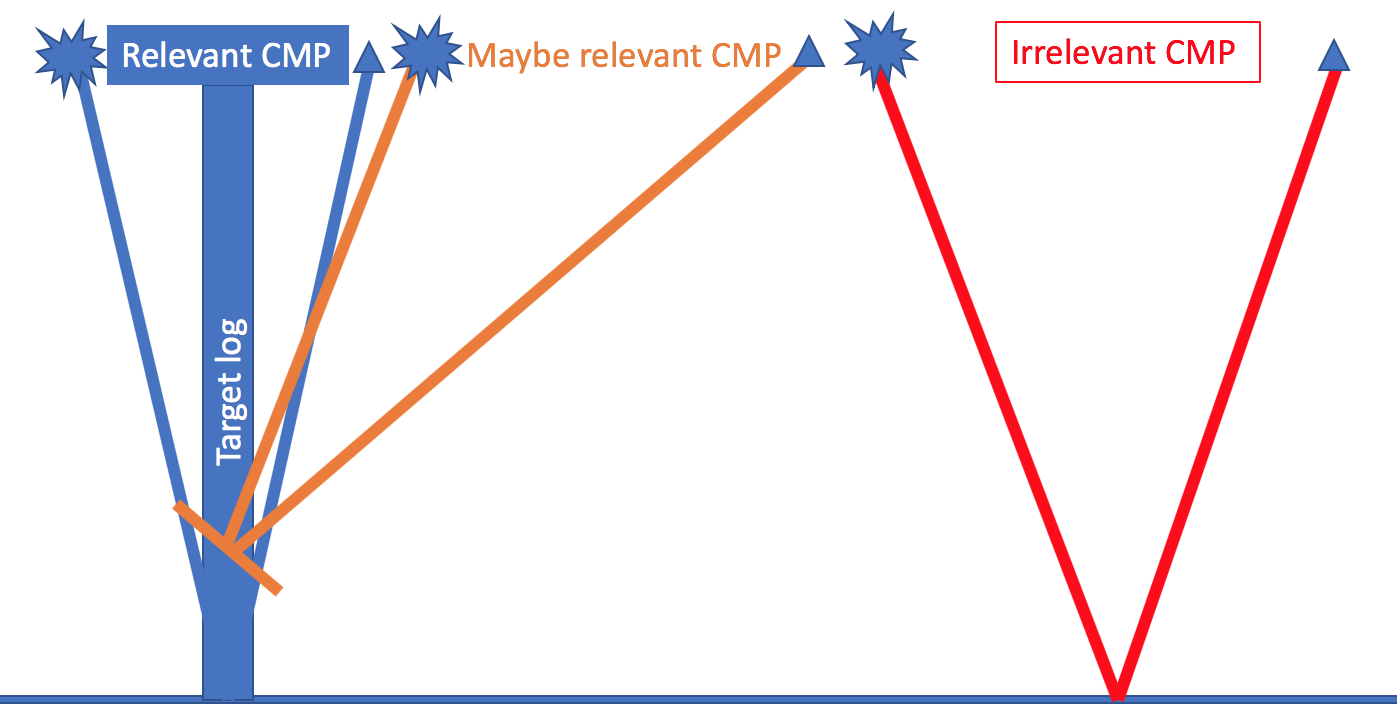
\includegraphics[width=0.7\linewidth]{Fig/relevantCMP}
	\caption{Relevant common mid point (CMP) gathers - right above the image point location are utilized by standard stacking procedures and FWI. The gathers that are slightly shifted may also be useful in laterally heterogeneous media, but they are often discarded. CMP gathers that are far away from the imaging point are not spatially related to the imaging point, we discard those from the input}
	\label{fig:relevantCMP}
\end{figure}

Standard velocity analysis does CMP stacking along hyperbolas and then the stacked data are mapped to depth. This obviously is good enough for horizontally layered media. More advanced velocity analysis techniques such as common reflection surface  \citep{mann1999common} or multifocusing \citep{gelchinsky1999multifocusing}, take care of mild horizontal velocity variations and curved reflectors relying on curtain assumptions about the subsurface. We take this concept to its extreme by relying on geologically plausible models as realistic scenarios and replacing the analysis with deep learning inference.

In particular, we construct CNN that is trained to perform mapping of relevant seismic data cubes to respective velocity logs \figref{in_out}: 
\beq \label{eq:mapping}
u_{obs}(x_{CMP}-\varepsilon:x_{CMP}+\varepsilon, h_{min}:h_{max}, :) \to v(x_{CMP}, :).
\eeq
Relevant observed data $u_{obs}(x_{CMP}-\varepsilon:x_{CMP}+\varepsilon, h_{min}:h_{max}, t)$  
to an estimate of velocity at target location $v(x_{CMP}, z)$, $x_{CMP}$ is the central midpoint,
$u_{obs}$ is the observed wavefield (acoustic pressure in our case). Here $x_{CMP}$ is the target vertical seismic velocity profile, $h_{min}$ and $h_{max}$ determine the shortest and the longest offsets that are usable from the data, $t$ and $z$ stand for time and depth respectively.

In the next subsection we discuss why mapping defined by \eqrf{mapping} would exist, and why it is a candidate for an optimal way to cast seismic exploration inverse problem in the deep learning set up.  
\begin{figure}[h!]
	\centering
	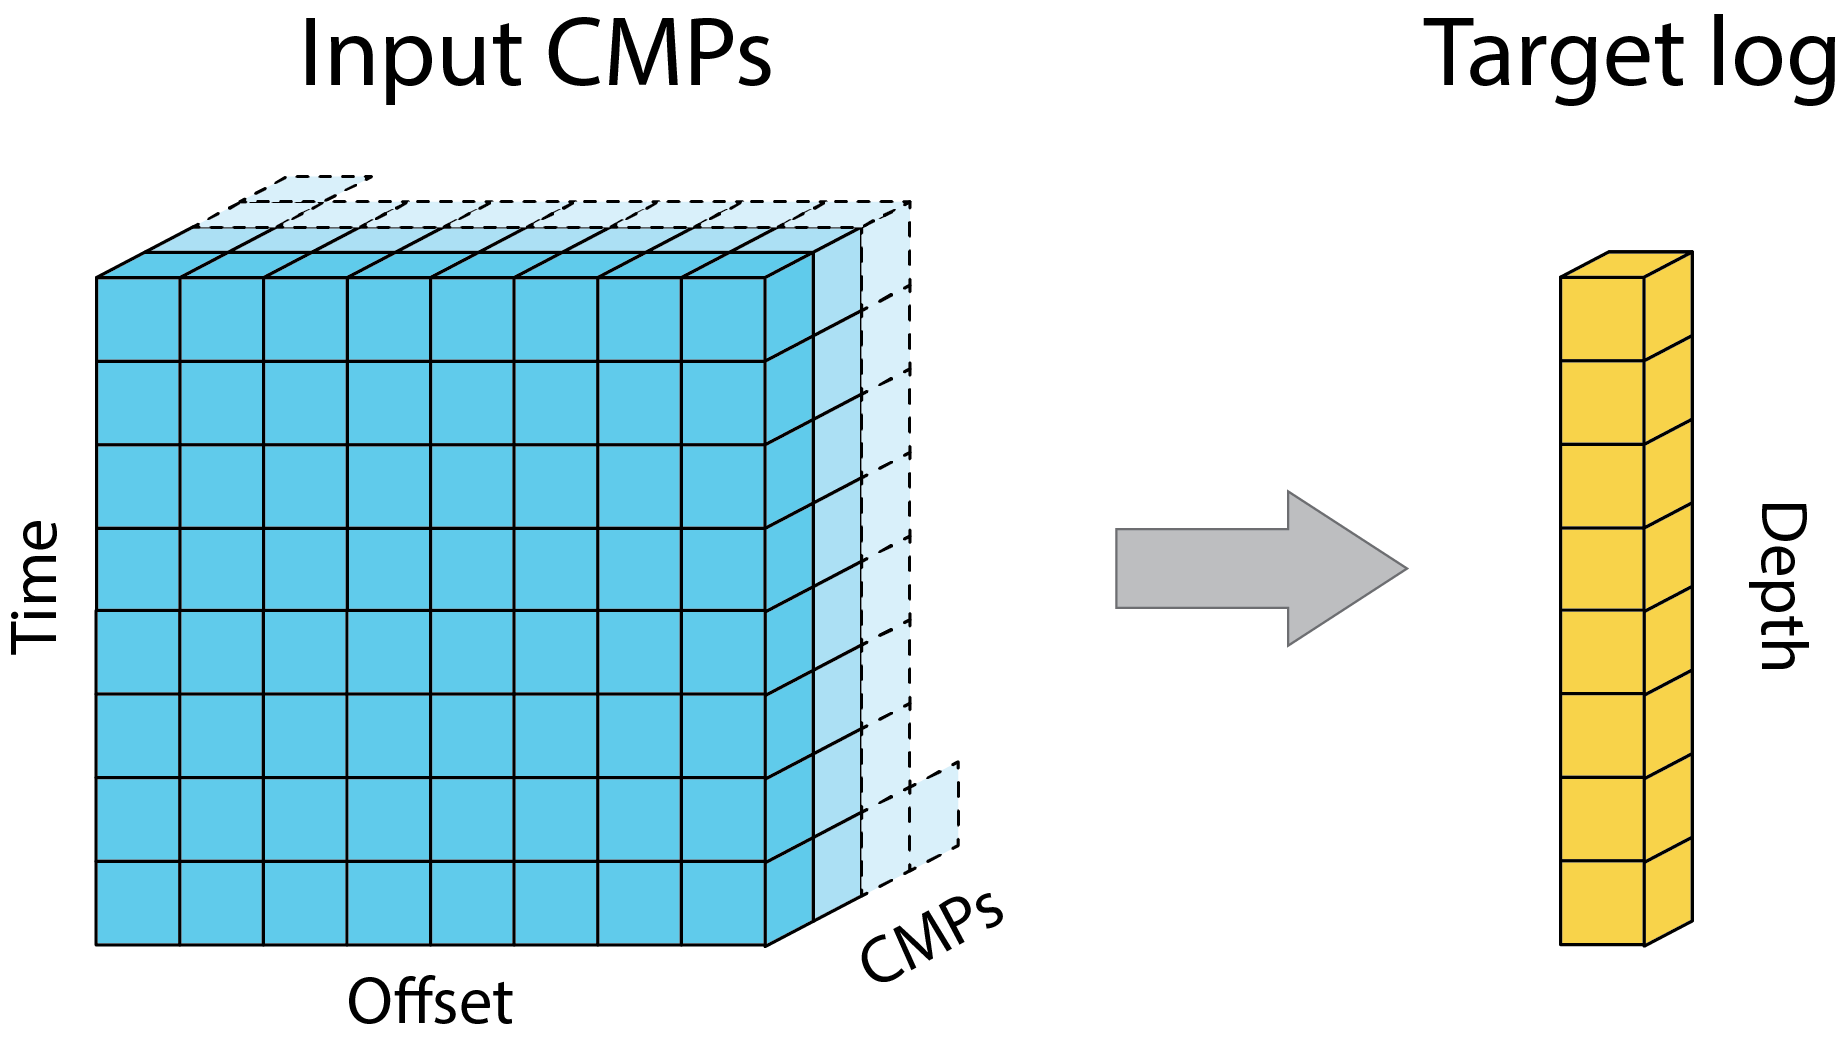
\includegraphics[width=0.7\linewidth]{Fig/in_out_shape}
	\caption{A set of neigboring CMP gathers is mapped to the velocity vertical profile with horizontal coordinate at the middle of this set}
	\label{fig:in_out}
\end{figure}

\subsection{Regularity of seismic data and deep learning inversion of full-waveforms}

Conventional active seismic acquisition aims at providing equal illumination to all the target areas of interest. This leads to the fact that data available at different spatial locations are typically very similar. Therefore it is natural to assume that the relations between the subsurface vertical profiles and data are similar regardless of the location. 

Moreover the acquisition is typically regularly sampled. Which means that from the experimental setup part the data available at a different location are identical. Therefore the problem of vertical velocity profile estimation is exactly the same regardless of the location for a given exploration field.

The resemblance between different location in the field of exploration is rather well understood and taken into account in seismic imaging methods that rely on simplified media assumptions, such as stacking. It however can not be easily incorporated into full-waveform modeling based methods such as FWI and reverse-time migration (RTM).   
%
Neural networks can serve as universal estimators therefore there is no principal constrainsts on which data space to map to which. Therefore they can be utilized to infer the mapping~\eqref{eq:mapping} from full-waveform modeling based methods. 

Finally, deep learning is typically very expensive computationally in the training part. From the mathematical point of view mapping~\eqref{eq:mapping} is a mapping of 3D functions (5D for the 3D data acquisition) on compact to 1D functions, which should theoretically be much easier to estimate than mapping of full data to full models which would need inference between 3D and 2D function in 2D problems, or even in 5D to 3D, for 3D problems. This makes mapping to 1D logs an affordable and sufficient option.

%The regularity of conventional seismic exploration data and exploit standard extended velocity analysis approach.

\section{Data}
Data-driven applications heavily depend on compound and quantity of samples in the dataset which makes data collection and selection crucial. 
%
We intend to produce virtual well-logs from seismic data arranged into common-midpoint gathers. The dataset for such application should consist of input seismic data and respective target logs. However, there is very limited amount of field samples on well-logs because drilling and collection of a core is a costly task. 
%
To overcome this limitation we generate a synthetic dataset representing real-world geological features. First, we generate a set of random initiations of subsurface models and then numerically propagate seismic waves in them. Later, recorded wavefields are assembled into CMPs and the random velocity models are decomposed into set of well logs.

\subsection{Pseudo-random models}
Despite the clarity of intention, there is still no a recognized way for generation of realistically textured all-purpose subsurface models with proper geological compound. 
%
We empirically generate pseudo-random subsurface models in three steps from the guiding model -- Marmousi benchmark model \citep{marmousi1991}.

\begin{itemize}
\item First, we build the geological prior by flipping and replicating the Marmousi model.

\item Then, we produce a distortion map from random Gaussian field \figref{deformedModelMild} and map vertical coordinates in the prior according to this field \figref{deformedModelNormal}. Similar kind of mild deformations are then utilized for data augmentation. 

%We then stretch coordinates further \figref{deformedModelNormal}.

\item Finally, we crop a random rectangular patch from the deformed model and resize it back to the size of the target subsurface model \figref{random_model_example}.
\end{itemize} 



%\dplot{stretchMarm}{stretchMarm_strip}{To generate a pseudo random model with realistic structures we first (a) flip and replicate Marmousi. (a) Full prior model. (b) Crop of the prior with dimensions similar to the original Marmousi II model.}

\dplot{deformedModelMild}{deformedModelNormal}{Generation of random subsurface models. Vertical shifts defined by random Gaussian field are applied to the geological prior. Before the transformation (a) and after (b).}
%Random Gaussian field defines (a) vertical shifts that we apply to the model. (b) deformed model

\aplot{random_model_example}{width=0.7\columnwidth}{An example of generated pseudo-random model.}


%\paragraph{Generator features}
The generator described above allows us to generate a set of models which to some extent mimic the layered geological structure from the Marmousi model. Despite using a specific velocity reference, the generator produces diverse range of subsurface models which then might be fit into desired range of velocities. The main part of the transformation is local texture vertical repositioning. However, depending on smoothness of coordinate transformation new horizontal layers can be generated and old layers collapsed.

\subsection{Seismic wave propagation}
There are no principal limitations to the type of wave equation or solver to be used. Yet, a few thousands of shots are necessary to generate statistically significant input for the machine learning. To reduce the computational costs of modeling acoustic 2D \citep{polo2018,ovcharenko2018,ovcharenko2019deep, li2019} or elastic 1D \citep[e.g.][]{zheng2019} solvers are typically utilized with relatively simple (small) models.

Should the model be horizontally invariant, one can try to reconstruct its elastic layers from a single shot gather \citep{roth1994}, or a single CMP gather \citep{zheng2019}.
While there is limited applicability to laterally inhomogeneous models \citep{zheng2019}, to the best of our knowledge, training was performed on vertically variant models to speed up the data generation. Here we utilize conventional finite-difference 2D wave propagation and investigate different options for laterally variant media.
Data are generated with equidistant sources and receivers at spacing of 100m. The maximum offset is limited to 4km and the source central frequency is set to 7Hz, to present a decent challenge to conventional FWI.

To generate seismic data in each random model we integrate the Madagascar package into the workflow. 
We use a CUDA-accelerated acoustic finite-difference solver in time domain to numerically simulate seismic wave propagation and to record seismograms at each receiver for every source in the acquisition.
%





% function "sfgenshots" - a cuda-based finite-difference solver. There are no principal limitations to the type of solver to be used. After that the shots are sorted into CMP gathers.

\section{Deep learning: Setup}
The general idea of deep learning is to build a mathematical model which would derive a desired non-linear relation directly from the data. Selection of a particular DL model is heavily motivated by the compound and attributes of the available data. 

%\subsection{Input and output}
%	supervised learning
We map multiple input CMP gathers (\figref{X_muted}) to respective target well-logs. Provided that the inputs and outputs are known, the problem reduces to multivariate regression. Therefore, the problem falls into the supervised learning setup.  

At the training stage, a supervised model attempts to derive a relation which would link input and target variable for each pair in the training partition of the dataset. Whereas at the inference stage, the model infers target variables when given a sample from previously unseen test partition of the data.

\subsection{Preprocessing}
Regardless of the type a DL model used in the application, proper normalization is required for each sample of the input and target data. Normalization makes data fit the range matching the bounds of activation functions as well as it enforces even contribution of features into training. All these leads weight optimization (training) to a better convergence at shorter time.

%Target data are seismic velocity profiles, those already have a range and have similar variability therefore standard Min-Max scaling to the into range $[-1, 1]$ works rather well for these data and does not change the patterns that can be extracted from those.  

Target data are seismic velocity profiles which naturally span a narrow range values and have similar variability. Therefore, common Min-Max scaling to the range $[-1, 1]$ enhances the target data representation while not changing the patterns that can be extracted from the logs.  

Input seismic data, on the other hand, require more complex geometric spreading correction.  Typically, the geometric correction leads to discontinuities in the data. Fortunately, studies on automatic gain control allow to overcome this issue and to preserve continuity in the data. 
%
We empirically found that standard Min-Max scaler from the Scikit-learn library \citep{scikit-learn}, applied to the set of samples, destroys spatial and temporal continuity in the data and leads to subsequently poor performance of the neural network. On the other hand, the standard scaler allowed us to preserve continuity in the data. After standard scaling, we downscale the data with empirically found coefficent of 0.1 and then mute the outliers to fit all the data into the [-1, 1] range (\figref{X_scaled}).

\dplot{X_muted}{X_scaled}{Input seismic data to the netwoek. Raw CMP gather (a) and scaled version of the same CMP gather (b). We utilize only positive offset as the data are synthetic and due to the reciprocity there is no difference with swaping source and receiver positions.}


\subsection{Convolutional neural networks (CNN)}
%   spatial dependency = convolutional
Regular feed-forward neural networks, such as multilayer perceptron, are suitable for problems with relatively small size of input data as the number of parameters in them grows exponentially. When the input volume is image then networks with convolutional layers come into play. Convolutional layers perform convolution of the input volume with a set of filters which results in a set of feature maps, one corresponding for each filter respectively. The key feature of convolutional layer is that it features local connectivity. Meaning that when the filter slides over the input volume, only very few neighboring points contribute into particular point of the feature map. This feature allows such a network to learn spatial patterns and enforce them at the inference stage.

Here, we consider two CNNs with exactly the same architecture, apart from the first layer which will accept input data of different shape.
%
First we construct a 2D convolutional neural network that shifts its filters along offset and time in individual CMPs. This neural network takes single CMP gather as input.
The second neural network takes multiple CMPs as multiple channels in the first layer and then follows exactly the same architecture as the first neural network \figref{architecture}.

%\subsection{CNN design}

\aplot{architecture}{width=\linewidth}{Purely convolutional neural architecture allows us to easily scale the input and output. Maximum pooling layer and layers with strides larger than one provide compression of the data within th neural network. \todo{Pavel will remake the fancy architecture plot}}


%	Preprocessing
%		explain preprocessing
%	explaing perks of conv 
%	keras tensorflow




%Here, following \citep{york2019}, we generate the data and try to learn the respective logs.

\section{DL: Training}
Fitting within the CNN happens through the filters. First, CNN filters are initialized with random numbers and then those are optimized to match the output. The optimization is typically executed with a local search method through backpropagation of errors of the neural network on training data set. 
%The network is trained given the training part of the dataset whereas its performance is estimated by evaluation of inference result on the validation data. Final performance is measured from inference on testing data.

\subsection{Data splitting}
The learning process starts with splitting all available data into training, validation and testing subsets. 
The goal of training is
%not learning the input-output relation as a data base or dictionary, but 
to infer the dependence between input and target data in a way that it can further be applied to other data. Therefore, the performance of the CNN is evaluated throughout the process of training by applying the neural network to so called validation data. Once CNN stops improving its performance on the validation data set the training stops. Hence, validation data is utilized in training for early stopping it would be unfair to test on those data. Thus a small portion of the data is isolated from the training procedure into the testing data set. 

Often the three subsets of the data are determined randomly, yet it is not fair in our case since samples are spatially correlated. If CNN has seen in the training has seen neighboring logs in the training all it does would be simple interpolation between those. To mitigate this problem in testing the neural network performance and in order to be able to see performance on training samples we split the data set in the following way. We extract last 20\% of samples and split them into 10\% for testing and 10\% that are used for every training that we perform throughout the paper. The rest 80\% of the data we split according to Pareto principle \citep{dunford2014pareto} into training and validation randomly \figref{T_data_split}. 


\subsection{Optimization}
Once the training set is organized one needs to choose the optimization strategy. This typically includes optimization algorithm and its parameters. We use one of the most popular optimizers in deep learning -- adaptive moment estimation enhanced by Nesterov accelerated momentum (Nadam, \cite{dozat2016incorporating}). We empirically find that batch size of 32 provides high, yet still stable performance over epochs in our case for about 30.000 samples \figref{singleCMP_loss_Full}. Nadam provides rapid decrease in the loss function and we notice that validation loss essentially stops decaying in about 20 epochs. Training takes about 5 seconds per epoch for the single CMP neural network and about 45 seconds for a single epoch for multi CMP neural network due to the large filter sizes in the first layer of the neural network.

\dplot{singleCMP_loss}{multiCMP_loss}{Loss functions on training and validation partitions of the dataset. Single CMP training (a) and multi CMP training (b).}

\subsection{Evaluation}
After training we can visually evaluate the performance of CNNs on the training and testing subsets of the initially generated data. Comparison of training results of single CMP CNN (\figref{train_singleCMP_predicted}), multi-CMP CNN (\figref{train_multiCMP_predicted}) and ground truth (\figref{train_multiCMP_true}) shows that both neural networks fit training data set fairly well, with mildly better fit by the multi CMP CNN. Also both neural networks seem to work well for the near-surface area in the models up to about 500m depth on testing data set. On the other hand the deeper structures are not that well revealed. Note, however, that taking into account the limited offset and central frequency of the wavelet conventional FWI would also probably fail for the deeper parts. %\todo{Quantitative comparison? Add any numbers}

\fplot{T_data_split}{train_singleCMP_predicted}
{train_multiCMP_predicted}{train_multiCMP_true}{(a) Velocity logs prepared for training and (b) scaled version for the CNN input. (c) Trained prediction from single CMP data, (d) from multi CMP data}

\subsection{Reproducibility}
One of the main features of the neural networks is their stochasticity. There are multiple reasonable mappings that the neural network could learn in the multidimensional regression setting. Leaving the randomness of our training data set out of scope (we fix the seed for reproducibility of the data set) stochasticity of the neural networks comes from several factors: random weight initiation, random training set shuffling, random parallel arithmetic operations order inside GPU. While first two factors could in principle be isolated by random seed selection, the third one is very hard to deal with and there is not much sense in particular choice of random initial weights for instance.

Therefore instead of going for exact numerical reproducibility we try to provide a clue about the randomness of our estimates by training multiple instances of our neural networks on the same data set. In order to keep computational time within few hours we take only five instances of each network, which is not enough to get a reasonable uncertainty estimate but provides us with some insights into it. In the next section we test our trained ensambles of five CNNs each.

\section{DL: Applications}
In most deep learning applications to seismic inverse problems the models are significantly simplified. Here we go for the full model complexity. The section consists of several synthetic test and is organized with increasing true model complexity. We start with a pseudo-1D model generated by horizontal stretching guiding model, then by random deformation of that model, which is still for the most part horizontally layered. After that we apply our inversion to the guiding Marmousi model itself. Then we examine application to a rescaled crop from SEAM model. Finally we show application to Overthrust model and its pseudo-1D derivative. In all our applications we postprocess the inversion results with median filter of size 700m horizontally and 150m vertically in order to reduce the deviation in predictions and reintroduce spatial relations between individual logs into the inversion.

%% figure naming convention:
%(train/test)_(prefix(singleCMP/multiCMP))_{folder(for train: ""=x1,x2,x3:marmvel1D, marmvel1D_distort,marmvel,overthrust1D,overthrust2D)}_{inverted/true/X_scaled}

\subsection{Guiding model and its derivatives}

Despite diversity of pseudo-random subsurface models used for training, these are still biased toward the guiding model which has been selected as prior. The purpose of this section is to investigate the behavior of the deep learning model when applied to different scenarios derived from the original guiding model.

\paragraph{Marmousi 1D}
\newcommand{\modelFname}{marmvel1D}

The first question that we would like to answer is if the CNN that we trained can f	it parts of the stretched Marmousi model that was utilized to make the training data set, yet were not used in training directly. \figref{test_singleCMP_\modelFname_true_Full} shows the results of inversion for synthetic data acquired in such a model. The model is essentially 1D and therefore as expected CNN utilizing single CMP input is performing better which is also reflected in the variance map \figref{test_singleCMP_\modelFname_inverted_std_dev} and \figref{test_multiCMP_\modelFname_inverted_std_dev}. The ensemble of CNNs is obviously not sufficient to estimate variance properly, yet we notice that the variance is increasing with depth and is focused around the layer location.
Data in this case are not significantly clipped (\figref{test_multiCMP_\modelFname_X_scaled}) and do not vary significantly between multi-CMP input channels.

\splot{test_singleCMP_\modelFname_true}{test_singleCMP_\modelFname_inverted}
{test_multiCMP_\modelFname_inverted}{test_singleCMP_\modelFname_inverted_std_dev}
{test_multiCMP_\modelFname_inverted_std_dev}{test_multiCMP_\modelFname_X_scaled}
{(a)Test model -- stretched crop from the left edge of the Marmousi model. Average prediction from the ensemble of (b) -- single CMP CNNs and (c) -- multi CMP CNN. Standard deviation for the (d) -- single CMP CNN outputs, (e) -- multi CMP CNN outputs. (f) Sample of input data rescaled with saved from the training process scaler for multi-CMP CNN (only first and last channels are displayed)}

\paragraph{Distorted Marmousi 1D}
\renewcommand{\modelFname}{marmvel1D_distort}
The second question is would it work better if we added more models generated just the way we generated our training data set. In order to do so we generate more models with the same generator and test whether the model can fit those already. We notice that shallow laterally varying anomalies can to some extent be estimated. The deeper par seems to be better resolved by multi-CMP CNN. Data representative in this case is not clipped much, but shows significant amplitude variation between multi-CMP channels.

\splot{test_singleCMP_\modelFname_true}{test_singleCMP_\modelFname_inverted}
{test_multiCMP_\modelFname_inverted}{test_singleCMP_\modelFname_inverted_std_dev}
{test_multiCMP_\modelFname_inverted_std_dev}{test_multiCMP_\modelFname_X_scaled}
{Same as \figref{test_singleCMP_marmvel1D_true_Full}, but for distorted 1D profile from Marmousi model. (e) The lateral heterogeneity becomes obvious in the CMP gathers}


\paragraph{Original Marmousi}
\renewcommand{\modelFname}{marmvel}
Guiding model -- Marmousi, was not directly added to the training set, but was used for the training set generation. It is largerly laterally heterogeneous, yet single CMP CNN provides a reasonable estimate, which would probably be good enough for subsequent FWI. The variance maps suggest that multi-CMP neural network provides a better estimate in this case.

\splot{test_singleCMP_\modelFname_true}{test_singleCMP_\modelFname_inverted}
{test_multiCMP_\modelFname_inverted}{test_singleCMP_\modelFname_inverted_std_dev}
{test_multiCMP_\modelFname_inverted_std_dev}{test_multiCMP_\modelFname_X_scaled}
{Same as \figref{test_singleCMP_marmvel1D_true_Full}, but for the Marmousi model itself}

\subsection{Generalization tests on other models}

Properly trained neural network should exhibit generalization capability. Meaning that it should infer meaningful result when applied to an unseen data. However, when the new input data is sufficiently different from the training data, prediction is expected to be inaccurate. In this paragraph, we demonstrate three applications of the network to the data significantly different from the one in training dataset. The first application is for salt-induced SEAM Phase I model, which produces data with strong reflections inconsistent with CMPs produced by a non-contrast training data. Other two examples are for 1D and 2D overthrust models which resemble layered structure of subsurface models used for training, however with different contrasts and layer inclination.


\paragraph{SEAM}
\renewcommand{\modelFname}{seam100}
SEAM Phase I model features strong reflections strong reflections inconsistent with CMPs produced by a non-contrast training data. This leads to poor standard scaler performance and a lot of data samples get clipped among the deeper reflections \figref{test_multiCMP_\modelFname_X_scaled}. On the other hand velocities in very near surface are low and diving waves don't get scaled properly. Some salt-like bodies are generated when we crop from deformed Marmousi model and stretch the crops. All these factors suggest that the training data set would need to be better tailored to local geology  therefore the inversion recovers only the velocity trends next to the salt and the salt boundary. FWI tailored to salt body inversion \citep[e.g.][]{esserTotalvariationRegularizationStrategies2016,ovcharenko2018,kalita2019regularized} would still benefit from such an estimate used as a starting model.

\splot{test_singleCMP_\modelFname_true}{test_singleCMP_\modelFname_inverted}
{test_multiCMP_\modelFname_inverted}{test_singleCMP_\modelFname_inverted_std_dev}
{test_multiCMP_\modelFname_inverted_std_dev}{test_multiCMP_\modelFname_X_scaled}
{Same as \figref{test_singleCMP_marmvel1D_true_Full}, but for the rescaled crop the SEAM model. (e) Scaling performs poorly as the training data set didn't include similar models}

Standard deviation maps describe inconsistency between log predictions by five identical but independent networks. These were trained starting from different weights initializations and thus converged to slightly distinct final weights. Central part of the deviation map dominates over the neighboring regions. This assumes that the network was not given sufficient amount of data on salt bodies. Meaning that it is not able to produce logs with large homogeneous high-velocity segments. 

\paragraph{Overthrust model}

In order to explore the generalization power of the trained neural network we test it on data that are modeled in a slice from the Overthrust model. Which is challenging for FWI due to its low velocity layers squeezed in between high velocity reflectors and also challenging for conventional layer stripping due to uplifts and faults that distort otherwise low-relief structure. We split the phenomena into two. First we replicate low-relief part of the Overthrust model to test the the layer stripping capabilities of the trained CNNs and then we test on the full model replicated and flipped.

\subparagraph{Overthrust 1D}
\renewcommand{\modelFname}{overthrust1D}

Shallower layers in this model feature low contrasts and velocity increases and then decreases \figref{test_singleCMP_\modelFname_true}. The data \figref{test_multiCMP_\modelFname_X_scaled} scaling shows very strong first arrivals and very low amplitude reflections, which focuses inversion on the near-surface anomalies.
Both CNNs seem to get the top of the model right \figref{test_singleCMP_\modelFname_inverted}
\figref{test_multiCMP_\modelFname_inverted} and fail at the bottom part. Single CMP CNN fails in a bit more moderate way as expected for this low-relief model. Deeper layers are mispositioned, which is reflected in overall increasing standard deviations within the ensembles \figref{test_singleCMP_\modelFname_inverted_std_dev} and
\figref{test_multiCMP_\modelFname_inverted_std_dev}. 

\splot{test_singleCMP_\modelFname_true}{test_singleCMP_\modelFname_inverted}
{test_multiCMP_\modelFname_inverted}{test_singleCMP_\modelFname_inverted_std_dev}
{test_multiCMP_\modelFname_inverted_std_dev}{test_multiCMP_\modelFname_X_scaled}
{Same as \figref{test_singleCMP_marmvel1D_true_Full}, but for the pseudo-1D model generated from Overthrust model}

\subparagraph{Overthrust 2D}
\renewcommand{\modelFname}{overthrust2D}
Both CNNs seem to get the top of the model right \figref{test_singleCMP_\modelFname_inverted}
\figref{test_multiCMP_\modelFname_inverted} and fail at the bottom part. Single CMP CNN fails in a bit more moderate way as expected for this low-relief model. Deeper layers are mispositioned, which is reflected in overall increasing standard deviations within the ensembles \figref{test_singleCMP_\modelFname_inverted_std_dev} and
\figref{test_multiCMP_\modelFname_inverted_std_dev}

Finally, we test both CNNs on a slice from the Overthrust model \figref{test_singleCMP_\modelFname_true}. The scaled data \figref{test_multiCMP_\modelFname_X_scaled} shows very strong first arrivals and very strong late reflections. Those reflections are most likely multiples and therefore it is very hard to train CNNs to position those properly. The latter probably leads to an anomaly in the left part of the inversion results  \figref{test_singleCMP_\modelFname_inverted}
\figref{test_multiCMP_\modelFname_inverted}. According to the standard deviation maps  \figref{test_singleCMP_\modelFname_inverted_std_dev} and
\figref{test_multiCMP_\modelFname_inverted_std_dev} up to the depth of 1.5km we can trust the inversions. However, only some features of the complicated layering are retrieved. We still expect that the inversion results would be useful as a starting point for FWI.

\splot{test_singleCMP_\modelFname_true}{test_singleCMP_\modelFname_inverted}
{test_multiCMP_\modelFname_inverted}{test_singleCMP_\modelFname_inverted_std_dev}
{test_multiCMP_\modelFname_inverted_std_dev}{test_multiCMP_\modelFname_X_scaled}
{Same as \figref{test_singleCMP_marmvel1D_true_Full}, but for the 2D slice of the Overthrust model}

%From the last test we clearly see a rather obvious fact -- single CMP gather can not be mapped into velocity log successfully without assumption of laterally slowly variant medium. We believe that this is a good motivation to study mapping of multiple CMP gathers.


\section{Conclusions}
For regularly sampled data acquisition the problem of full waveform inversion can be represented as a mapping from 3D data (relevant traces) to single velocity logs. This formulation is not a viable option for conventional FWI implementation. Yet for neural network implementation it is beneficial to split whole data set into relevant and irrelevant data to speed up training.  
We analyzed the capabilities of CNNs to infer the relation between the data and vertical velocity slices. For very slowly varying laterally models the fitting by single CMP -- single velocity log works rather well and there is no need for multi-CMP processing. However for realistically varying with offset models there is need for multi-CMP input as single-CMPs can not be mapped into complex structures. Extending realistic training datasets is necessary to improve performance of more sophisticated inversions with CNNs.


\section{ACKNOWLEDGMENTS}

We thank members of the Seismic Modeling and Inversion group (SMI) and the Seismic Wave Analysis Group (SWAG) at KAUST for constructive discussions. We also thank Saudi Aramco for support.
The research reported in this publication was supported by funding from King Abdullah University of Science and Technology (KAUST), Thuwal, 23955-6900, Saudi Arabia.

%\append{Appendix example}



\newpage

\bibliographystyle{apalike}  % style file is seg.bst
\bibliography{zotero}

\end{document}